% @Author: AnthonyKenny98
% @Date:   2020-04-04 11:13:58
% @Last Modified by:   AnthonyKenny98
% @Last Modified time: 2020-04-04 12:09:59
% @Author: AnthonyKenny98
% @Date:   2020-02-29 17:30:44
% @Last Modified by:   AnthonyKenny98
% @Last Modified time: 2020-04-03 14:28:30
\begin{figure}[H]
\begin{center}
\begin{tabular}{cc}

    % Subfigure A
    \begin{subfigure}{0.4\textwidth}
    \begin{center}
    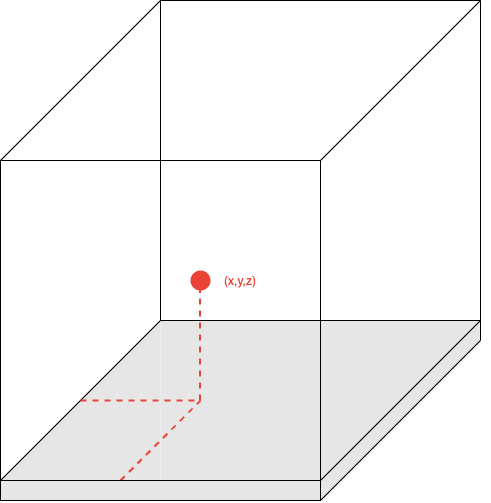
\includegraphics[width=\linewidth]{chapters/chapter2/img/motionPlanning/3DPointConfiguration.png}
    \caption{A robot represented by just a point in 3D space, requiring only 3 Cartesian coordinate $(x,y,z)$ points to describe its \gls{configuration}}
    \label{subfig:3DPointConfig}
    \end{center}
    \end{subfigure}
    &
    % 
    % Subfigure B
    \begin{subfigure}{0.4\textwidth}
    \begin{center}
    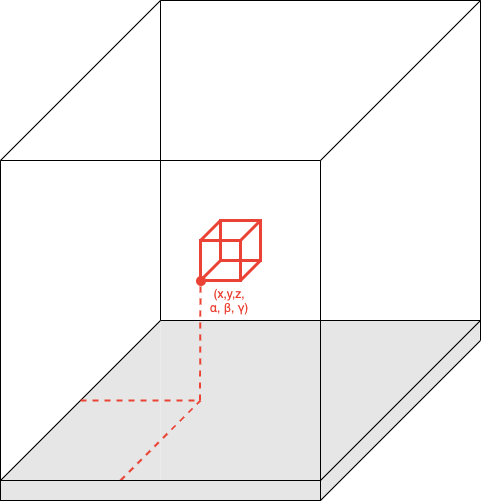
\includegraphics[width=\linewidth]{chapters/chapter2/img/motionPlanning/3DCubeConfiguration.png}
    \caption{A robot represented as a cube in 3D space, now requiring 3 Euler angles $(\alpha, \beta, \gamma)$ along with the original Cartesian coordinates.}
    \label{subfig:3DCubeConfig}
    \end{center}
    \end{subfigure} \\
\end{tabular}
    % Caption and Label
    \caption{Example of 2 Robot Configurations in 3D Space for Motion Planning Purposes}
    \label{fig:configuration}

\end{center}
\end{figure}